\lecture{Deterministic Finite Automata}{14:00}{09/02/24}{Jiacheng Tan}

Rather than regular expressions, you can use state transition diagrams to describe patterns, or the process of matching
 said patterns. State transition diagrams (or state diagrams) are directed graphs which represent Finite State Automata
 (FSA) or Finite Automata (FA)

\section*{FSA}

An FSA has
\begin{itemize}
  \item A set of states
  \item A unique start state
  \item A set of one or more final/accepting states
  \item An input alphabet, including a unique symbol to represent the end of the input string
  \item A state transition function, represented by the edges of a directed graph from one state to another, labelled by
   one or more symbols of the alphabet
\end{itemize}

Mathematically speaking, an FSA $M$ consists of
\begin{itemize}
  \item A finite set, $Q$, of states
  \item A finite alphabet, $\Sigma$ of input symbols
  \item A unique start state, $q_1 \in Q$
  \item A set of one or more final/accepting states, $F \in Q$
  \item A transition function $\delta : Q \times \Sigma \rightarrow Q$ which selects a new state for $M$ based on the
   current state, $s \in Q$ and the current input symbol $a \in \Sigma$
\end{itemize}

\subsection*{DFAs and NFAs}

A finite automata can be either deterministic (DFA) or non-deterministic (NFA). For a FA to be deterministic, it must
 perform the exact same state transition in a given situation (it's current state and input). If the FA is
 non-deterministic, it can perform any state transition in a given situation

\section*{DFAs for Lexical Analysis}

In the context of lexical analysis, a DFA is a string processing machine, using the following process, being in one of a
 finite set of states at any given step
\begin{itemize}
  \item Read a string from left to right, one symbol at a time
  \item On reading a symbol, move to a new state determined by the current state and the symbol which was read
  \item Upon reading the final symbol, if the current state is an accepting state, then the string is valid. If not, the
   string is invalid
\end{itemize}

\section*{Transition Diagrams}

A DFA is usually represented using a transition diagram. This is a directed graph in which each node represents a
 possible state, and each edge a transition between states. The label for each edge determines what input character is
 required for the transition to take place. The DFA begins in the initial state, represented by the small arrow pointing
 into state 1. Each edge is labelled with the character required to make that transition, such as requiring an `a' to
 transition from state 1 to 2. Transitions can move to another state, or return to themselves. The accepting state, 4,
 is represented by a double circle.

\begin{figure}[h]
  \centering

  \usetikzlibrary{automata, positioning, arrows}
  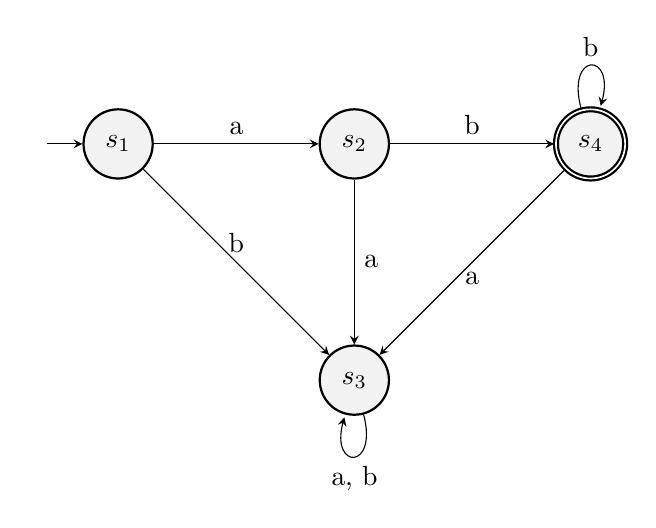
\begin{tikzpicture}
    \tikzset{
      ->, % makes the edges directed
      >=stealth, % makes the arrow heads bold
      node distance=3cm, % specifies the minimum distance between two nodes
      every state/.style={thick, fill=gray!10}, % sets the properties for each ’state’ node
      initial text=$ $, % sets the text that appears on the start arrow
    }

    \node[state] (s2) {$s_2$};
    \node[state, initial, left of=s2] (s1) {$s_1$};
    \node[state, below of=s2] (s3) {$s_3$};
    \node[state, accepting, right of=s2] (s4) {$s_4$};

    \draw (s1) edge[above] node{a} (s2)
          (s1) edge[above] node{b} (s3)
          (s2) edge[right] node{a} (s3)
          (s2) edge[above] node{b} (s4)
          (s3) edge[loop below] node{a, b} (s3)
          (s4) edge[below] node{a} (s3)
          (s4) edge[loop above] node{b} (s4);
  \end{tikzpicture}

  \caption{A simple DFA, $M$, which uses the alphabet $\Sigma = \{a, b\}$}
\end{figure}

For this DFA, the equivalent regular expression could be either $r = abb^*$ or $r = ab^+$. In the case of the transition
 diagram above, the DFA would be defined as
\begin{itemize}
  \item $Q = \{s_1, s_2, s_3, s_4\}$ is the set of states
  \item $\Sigma = \{a, b\}$ is the DFA's input alphabet
  \item $q_1 = s_1, \in Q$ is the initial state
  \item $F = \{s_4\}$ is the set of accepting states
  \item The transition function can be represented as the following set of triples:\\
  $\{(s_1, a, s_2), (s_1, b, s_3), (s_2, a, s_3), (s_2, b, s_4), (s_3, \{a, b\}, s_3), (s_4, a, s_3), (s_4, b, s_4)\}$
\end{itemize}

\subsection*{Languages}

The set of all strings which a DFA accepts is known as it's recognised language. For a DFA, $M$, the language, $L(M)$ is
 defined as the set of all strings $w \in \Sigma^*$ such that, when the DFA starts processing $w$ from it's initial
 state, it ends up in an accepting state. For example, the language, $L(M)$ of the DFA above could be defined as
 $L(M) = \{ab^n \mid n \geq 1\}$, and therefore is the same as the regular expression $r = ab^+$. For any regular
 expression, $r$, there is a DFA or NFA, $M$, such that $L(r) = L(M)$. This makes DFAs and transition diagrams very
 useful for creating regular expressions, and testing that they work as intended.

\subsection*{Simplifying Transition Diagrams}

Since most regular expressions, and therefore FAs, work with real languages such as English, each transition may have
 many characters for which it is valid. For example, a letter match would require 52 characters, one for each lower-case
 and capital letter. For this reason, as with regular expressions, you can define a set of symbols which are then used
 to label each transition, without rewriting the entire set of characters each time.

\section*{Building a Lexical Analyser}

Lexical analysers tend to be built using one of three methods
\begin{itemize}
  \item Write the formal description, e.g. a regular expression, of the token patterns, then use this as an input to
   a program such as \textbf{Lex}, which automatically generates a lexical analyser based upon the input
  \item Design DFAs which describe the patterns, then write a program to implement the DFAs
  \item Design DFAs which describe the patterns, then write a table-driven implementation of the DFAs
\end{itemize}
There are also algorithms which can be used to automatically construct a lexical analyser from the DFAs

\subsection*{Lex}

Lex was originally written in the 70s, but since then several variants have been created, such as Quex which is a much
 faster implementation of the same algorithms, written in C and C++. The program takes an input file, called a lex file,
 which contains regular expressions for various tokens, and automatically generates the C source code for a lexical
 analyser.

In it's most basic form, a Lex file consists of a series of lines in the form \verb`pattern action`, where pattern is a
 regular expression which should be matched, and action is a piece of C code.